%% This Beamer template is based on the one found here: https://github.com/sanhacheong/stanford-beamer-presentation, and edited to be used for Stanford ARM Lab

\documentclass[10pt]{beamer}
%\mode<presentation>{}

\usepackage{media9}
\usepackage{amssymb,amsmath,amsthm,enumerate}
\usepackage{mathtools}
\usepackage[utf8]{inputenc}
\usepackage{array}
\usepackage[parfill]{parskip}
\usepackage[utf8]{vietnam}
\usepackage{graphicx,animate}
\usepackage{caption}
\usepackage{subcaption}
\usepackage{bm}
\usepackage{amsfonts,amscd}
\usepackage[]{units}
\usepackage{listings}
\usepackage{multicol}
\usepackage{multirow}
\usepackage{tcolorbox}
\usepackage{physics}
\usepackage{movie15}
% Enable colored hyperlinks
\hypersetup{colorlinks=true}

\usefonttheme{professionalfonts}

% The following three lines are for crossmarks & checkmarks
\usepackage{pifont}% http://ctan.org/pkg/pifont
\newcommand{\cmark}{\ding{51}}%
\newcommand{\xmark}{\ding{55}}%

% Numbered captions of tables, pictures, etc.
\setbeamertemplate{caption}[numbered]
\usepackage{media9} 
%\usepackage[superscript,biblabel]{cite}
%\usepackage{algorithmic}
%\usepackage{algorithm2e}
%\usepackage{algpseudocode}
\usepackage[linesnumbered,ruled,vlined]{algorithm2e}
%\usepackage{algorithm}
%\usepackage{algorithmic}
%\usepackage{caption}
\usepackage[font=scriptsize,justification=centering]{caption}
%\usepackage{xcolor}
\usepackage{array}
%\renewcommand{\thealgocf}{}

\usepackage[natbib,backend=biber,style=ieee, sorting=ynt]{biblatex}
\bibliography{ref.bib}

\usepackage[acronym]{glossaries}

\usepackage{graphicx}
\graphicspath{{./figures}}
\usepackage{hyperref}

\usepackage{pythonhighlight}

\setbeamertemplate{theorems}[numbered]
\theoremstyle{remark}
\newtheorem{dl}{Định lý}
\newtheorem{md}{Mệnh đề}
\newtheorem{bd}{Bổ đề}
\newtheorem{dn}{Định nghĩa}
\newtheorem{hq}{Hệ quả}
%\theoremstyle{definition}

\numberwithin{algocf}{section}
\numberwithin{equation}{section}
\numberwithin{dl}{section}
\numberwithin{figure}{section}


%\newcommand{\empy}[1]{{\color{darkorange}\emph{#1}}}
%\newcommand{\empr}[1]{{\color{cardinalred}\emph{#1}}}
%\newcommand{\examplebox}[2]{
%\begin{tcolorbox}[colframe=darkcardinal,colback=boxgray,title=#1]
%#2
%\end{tcolorbox}}

%\usetheme{Stanford} 
%\input{./style_files_stanford/my_beamer_defs.sty}
\usetheme{Copenhagen}
\usecolortheme{seahorse}
%\logo{
\includegraphics[height=0.5in]{logos/HUS-name.jpg}}

\makeatletter
\let\@@magyar@captionfix\relax
\makeatother

\title[Kiến trúc lập trình song song và phân tán]{Kiến trúc lập trình song song và phân tán với OpenMP - MPI - CUDA}

\AtBeginSection[]
{
    \begin{frame}
        \frametitle{Nội dung}
        \tableofcontents[currentsection, subsectionstyle=show/show/hide]
    \end{frame}
}

\setbeamertemplate{page number in head/foot}[totalframenumber]
\setbeamertemplate{frametitle continuation}{}

\begin{document}
\author[Nguyễn Chí Thanh - 21007925]{
	\begin{tabular}{c} 
	\Large
	Nguyễn Chí Thanh \\
    \footnotesize \href{mailto:nguyenchithanh\_sdh21@hus.edu.vn}{nguyenchithanh\_sdh21@hus.edu.vn}
\end{tabular}
\vspace{-4ex}}

\institute{
	\vskip 5pt
	\begin{figure}
		\centering
		\begin{subfigure}[t]{0.5\textwidth}
			\centering
			
\includegraphics[height=0.75in]{logos/HUS-logo.jpg}
		\end{subfigure}%
		~ 
		\begin{subfigure}[t]{0.5\textwidth}
			\centering
			
\includegraphics[height=0.75in]{logos/MIM-logo.png}
		\end{subfigure}
	\end{figure}
	\vskip 5pt	
	Đại học Quốc Gia Hà Nội \\
	Trường đại học Khoa học tự nhiên\\
	Khoa Toán - Cơ - Tin học
	\vskip 3pt
}

%\begin{noheadline}
\begin{frame} \maketitle \end{frame}
%\end{noheadline}
    
\setbeamertemplate{itemize items}[default]
\setbeamertemplate{itemize subitem}[circle]

\begin{frame}{Nội dung}
    \tableofcontents[hidesubsections]
\end{frame}

\section{OpenMP}

\begin{frame}{Giới thiệu OpenMP}
    \begin{itemize}
        \item OpenMP là một API viết các ứng dụng đa luồng bộ nhớ chia sẻ sử dụng ngôn ngữ C/C++ hoặc Fortran
        \item Gồm có các chỉ thị biên dịch, runtime routine, biến môi trường.
        \item Hội đồng phát triển và phê duyệt kiến trúc OpenMP:
        \begin{itemize}
            \item Duy trì spec OpenMP
            \item Thành viên chính: AMD, Cray, Fujitsu, HP, IBM, Intel, Oracle, NVIDIA, Microsoft, Tesxas Instruments, Convey
            \item Thành viên ngắn hạn: ANL,	ASC/LLNL, cOMPunity, EPCC, LANL, NASA, TACC, RWTH, Aachen University, UH
        \end{itemize}
    \end{itemize}
\end{frame}

\begin{frame}{Các thành phần của OpenMP}
    \begin{columns}[onlytextwidth]
        \begin{column}{0.3\textwidth}
            Các chỉ thị biên dịch:
            \begin{itemize}
                \item Parallel region	
                \item Worksharing constructs
                \item Tasking
                \item Offloading
                \item Affinity
                \item Error Handling
                \item SIMD
                \item Synchronization
                \item Data-sharing attributes
            \end{itemize}
        \end{column}
        \begin{column}{0.3\textwidth}
            Các biến runtime:
            \begin{itemize}
                \item Số luồng
                \item Thread ID 
                \item Dynamic thread adjustment
                \item Nested parallelism
                \item Schedule
                \item Active levels
                \item Thread limit
                \item Nesting level
                \item Ancestor thread
                \item Team size 
                \item Locking
                \item Wallclock timer
            \end{itemize}
        \end{column}
        \begin{column}{0.3\textwidth}
            Các biến môi Trường:
            \begin{itemize}
                \item Số luồng
                \item Scheduling type
                \item Dynamic thread adjustment
                \item Nested parallelism
                \item Stacksize
                \item Idle threads
                \item Active levels
                \item Thread limit
            \end{itemize}
        \end{column}
    \end{columns}
\end{frame}

\begin{frame}
    \begin{figure}[H]
        \centering
        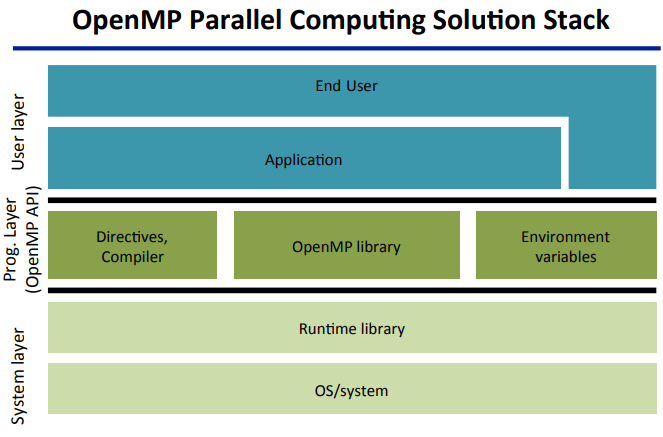
\includegraphics[width=0.9\linewidth]{figures/OpenMP/OpenMP_Parallel_Computing_Solution_Stack.png}
        \caption{Vị trí OpenMP trong stack}
    \end{figure}
\end{frame}

\begin{frame}{Chỉ thị biên dịch}
    \begin{itemize}
        \item Chỉ thị thực thi OpenMP áp dụng cho các khối có cấu trúc đứng kế tiếp với nó.
        \item Một chỉ thị bắt đầu với \#pragma omp. Các phần còn lại tuân theo quy ước của ngôn ngữ C và C++ cho các chị thị biên dịch 
    \end{itemize}
\end{frame}

\begin{frame}{Một số chỉ thị biên dịch của OpenMP}
    \begin{itemize}
        \item \#pragma omp parallel
        \item \#pragma omp for
        \item \#pragma omp sections
        \item \#pragma omp parallel shared/private
        \item \#pragma omp barrier
    \end{itemize}
\end{frame}

\begin{frame}{Mô hình thực thi Fork-Join của OpenMP}
    \begin{figure}[H]
        \centering
        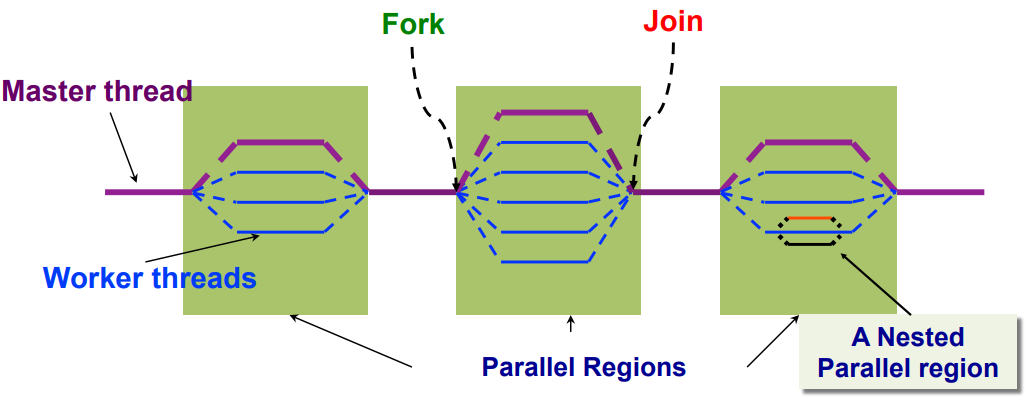
\includegraphics[width=\linewidth]{figures/OpenMP/Fork_Join_Execution_Model.png}
        \caption{Mô hình thực thi Fork-Join của OpenMP}
    \end{figure}
\end{frame}

\begin{frame}{Mô hình bộ nhớ của OpenMP}
    \begin{columns}[onlytextwidth]
        \begin{column}{0.5\linewidth}
            \begin{figure}[H]
                \centering
                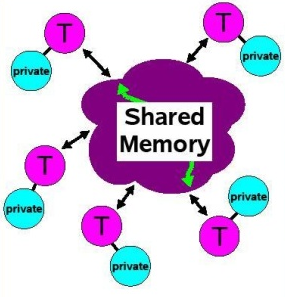
\includegraphics[width=\linewidth]{figures/OpenMP/OpenMP_Shared_Memory_Model.png}
            \end{figure}
        \end{column}
        \begin{column}{0.5\linewidth}
            \begin{itemize}
                \item Tất cả các luồng có cùng bộ nhớ chia sẻ toàn cục.
                \item Dữ liệu có thể chia sẻ hoặc riêng tư giữa các luồng
                \item Dữ liệu chia sẻ có thể truy cập từ tất cả các luồng
                \item Dữ liệu riêng tư chỉ có thể được truy cập từ luồng sở hữu dữ liệu
                \item Chia sẻ dữ liệu trong suốt với lập trình viên
                \item Có đồng bộ hóa, chủ yếu ngầm diễn ra.
            \end{itemize}
        \end{column}
    \end{columns}
    
\end{frame}

\begin{frame}[fragile]{OpenMP parallel region}
    Trong C/C++: một khối là một biểu thức hoặc một nhóm biểu thức giữa cặp ngoặc { }.
    \begin{columns}[onlytextwidth]
        \begin{column}{0.5\linewidth}
            \begin{verbatim}
#pragma omp parallel
{
    id = omp_get_thread_num();
    res[id] = lots_of_work(id);
}
            \end{verbatim}
        \end{column}
        \begin{column}{0.5\linewidth}
            \begin{verbatim}
#pragma omp parallel for
for(i=0;i<N;i++) {
    res[i] = big_calc(i);
    A[i] = B[i] + res[i];
} 
            \end{verbatim}
        \end{column}
    \end{columns}
\end{frame}

\begin{frame}{Chạy thực thi}
    \begin{itemize}
        \item Đặt biến môi trường OMP\_NUM\_THREADS.
        \item Chạy lệnh: g++ -fopenmp -g ./input.c -o ./input
    \end{itemize}
\end{frame}

\begin{frame}[fragile]{Chương trình đơn giản OpenMP}
    \begin{verbatim}
        #include <stdio.h>
        #include <omp.h>

        int main(int argc, char** argv) {
            #pragma omp parallel
            {
                printf("Hello World\n");
            } // End of parallel region 
            return 0;
        }
    \end{verbatim}
    Thực thi chương trình:
    \begin{verbatim}
        g++ -fopenmp -g ./hello_openmp.c -o ./hello_openmp
        ./hello_openmp
    \end{verbatim}
\end{frame}

\begin{frame}[fragile]{Khối lệnh có cấu trúc}
    \begin{itemize}
        \item Khối lệnh có cấu trúc: Một điểm vào và một điểm ra.
        \item Trong C/C++: một khối lệnh là một câu lệnh đơn hoặc một nhóm các câu lệnh giữa các ngoặc.
    \end{itemize}

    \begin{columns}[onlytextwidth]
        \begin{column}{0.5\textwidth}
            \begin{verbatim}
#pragma omp parallel
{
id = omp_get_thread_num(); 
A[id] = big_compute(id);
}		
            \end{verbatim}
        \end{column}
        \begin{column}{0.5\textwidth}
            \begin{verbatim}
#pragma omp for
for (int i=0;i<N;i++) {
    res[i] = big_calc(i);
    A[i] = B[i] + res[i]; 
}
            \end{verbatim}
        \end{column}
    \end{columns}
\end{frame}

\begin{frame}[fragile]{Cách viết rút gọn chỉ thị}
    Hai cách viết sau là tương đương:
    \begin{columns}[onlytextwidth]
        \begin{column}{0.5\textwidth}
            \begin{verbatim}
int i;
double res[MAX];
#pragma omp parallel				
{
    #pragma omp for
    for (i=0;i< MAX; i++) {
        res[i] = huge();
    } 
}
            \end{verbatim}
        \end{column}
        \begin{column}{0.5\textwidth}
            \begin{verbatim}
int i;
double res[MAX];
#pragma omp parallel for					
for (i=0;i< MAX; i++) {
    res[i] = huge();
}
            \end{verbatim}
        \end{column}
    \end{columns}
\end{frame}

\begin{frame}[fragile]{Đặt số luồng thực thi}
    Cách 1:
    \begin{verbatim}
export OMP_NUM_THREADS=4
    \end{verbatim}
    Cách 2:
    \begin{verbatim}
omp_set_num_threads(4);
    \end{verbatim}
\end{frame}

\begin{frame}[fragile]{Minh họa quá trình chạy song song}
    \begin{columns}[onlytextwidth]
        \begin{column}{0.5\textwidth}
            \begin{verbatim}
...A... 
#pragma omp parallel
{
    foo(); /* ...B... */
}
...C... 
#pragma omp parallel
{
...D...
}
...E...
            \end{verbatim}
        \end{column}
        \begin{column}{0.5\textwidth}
            \begin{figure}[H]
                \centering
                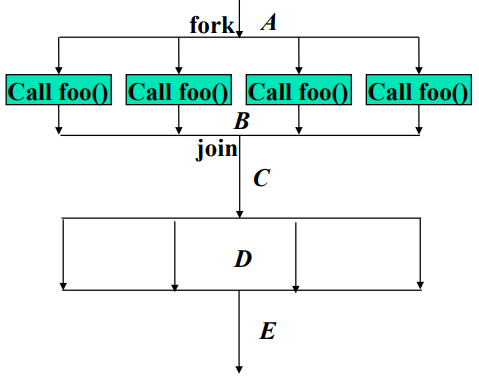
\includegraphics[width=\linewidth]{figures/OpenMP/Fork.png}
            \end{figure}
        \end{column}
    \end{columns}
\end{frame}

\begin{frame}[fragile]{Nguyên lý thiết kế}
    \begin{verbatim}
#pragma omp parallel
{
    int thread_id = omp_get_thread_num();
    int num_threads = omp_get_num_threads();
    printf("Thread %d of %d\n", thread_id, num_threads); 
}
    \end{verbatim}
    \begin{itemize}
        \item Từng hàm printf() là một tác vụ
        \item Parallel region tập hợp một tập các luồng cho tính toán và xử lý.
        \item Từng luồng thực thi một tác vụ đơn lẻ
        \item Ánh xạ 1:1 giữa các tác vụ và luồng
    \end{itemize}
\end{frame}

\begin{frame}[fragile]{Cú pháp OpenMP}
    \begin{itemize}
        \item OpenMP sử dụng các chỉ thị biên dịch dạng \#pragma.
        \item Với C và C++, chỉ thị có dạng:
        \begin{verbatim}
#pragma omp construct [clause [clause]...]
        \end{verbatim}
        \item Khai báo tệp tiêu đề: \#include <omp.h>
    \end{itemize}
\end{frame}

\begin{frame}[fragile]{Mô hình chương trình SIMD}
    \begin{itemize}
        \item SIMD cho parallel region:
        \begin{itemize}
            \item Tất cả các luồng của parallel region cùng thực thi một đoạn code.
            \item Mỗi luồng có một ID riêng
        \end{itemize}
        \item Có thể sử dụng threadID để phân nhánh thực thi các luồng, các luồng khác nhau có thể theo những con đường khác nhau qua cùng đoạn code:
        \begin{verbatim}
if(thread_id == x) {

} else {

}
        \end{verbatim}
        \item SIMD được sử dụng rất phổ biến cho cấu trúc các chương trình song song: OpenMP, MPI, CUDA,...
    \end{itemize}
\end{frame}

\begin{frame}[fragile]{Phân nhánh parallel regions}
    Chỉ có luồng master in ra màn hình số luồng
        \begin{verbatim}
#pragma omp parallel
 {
    int thread_id = omp_get_thread_num(); 
    int num_threads = omp_get_num_threads();
    if (thread_id == 0) 
        printf("Thread %d of %d\n", thread_id, num_threads); 
    else 
        printf("Thread %d\n", thread_id);
 }
        \end{verbatim}
\end{frame}

\begin{frame}[fragile]{Phân nhánh parallel regions}
    Chỉ có luồng master đọc số luồng và tất cả các luồng cùng in ra số luồng
    \begin{verbatim}
#pragma omp parallel
{
    int thread_id = omp_get_thread_num();
    if (thread_id == 0)
        num_threads = omp_get_num_threads();
    #pragma omp barrier
    printf("Thread %d of %d\n", thread_id, num_threads); 
}
    \end{verbatim}
\end{frame}

\begin{frame}{Chỉ thị Barrier}
    \begin{figure}[H]
        \centering
        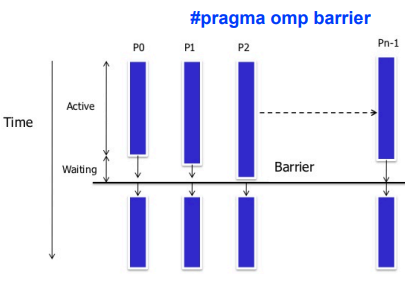
\includegraphics[width=0.9\linewidth]{figures/OpenMP/Barrier.png}
        \caption{Đồng bộ hóa giữa các luồng}
    \end{figure}
\end{frame}

\begin{frame}[fragile]{Chỉ thị Barrier}
    \begin{verbatim}
#pragma omp parallel shared (A, B, C) private(id)
{
    id=omp_get_thread_num();
    A[id] = big_calc1(id);
    #pragma omp barrier
    #pragma omp for
    for(i = 0;i < N; i++){
        C[i] = big_calc3(I, A);
    }
    // Có một barrier ngầm định kết thúc vòng lặp for
    #pragma omp for nowait // loại bỏ barrier
    for(i=0; i < N; i++){ 
        B[i] = big_calc2(C, i); 
    }
    A[id] = big_calc3(id);
} // Một barrier ngầm định kết thúc parallel region
    \end{verbatim}
\end{frame}

\begin{frame}[fragile]{Chỉ thị master}
    \begin{itemize}
        \item Ký hiệu khối lệnh chỉ được thực thi bởi luồng master
        \item Các luồng khác bỏ qua
        \item Không có đồng bộ hóa ngầm định
    \end{itemize}
    \begin{verbatim}
#pragma omp parallel private (tmp)
{
    do_many_things_together();
    #pragma omp master
    { 
        exchange_boundaries_by_master_only (); 
    }
    #pragma barrier
    do_many_other_things_together();
} 
    \end{verbatim}
\end{frame}

\begin{frame}[fragile]{Chỉ thị single}
    \begin{itemize}
        \item Ký hiệu khối lệnh chỉ được thực thi bởi một luồng
        \item Một barrier được ngầm định ở cuối khối lệnh
    \end{itemize}
    \begin{verbatim}
#pragma omp parallel private (tmp)
{
    do_many_things_together();
    #pragma omp single
    { 
        exchange_boundaries_by_one(); 
        }
    do_many_other_things_together();
}
    \end{verbatim}
\end{frame}

\begin{frame}[fragile]{Phân chia công việc sử dụng thread id}
    \begin{figure}[H]
        \centering
        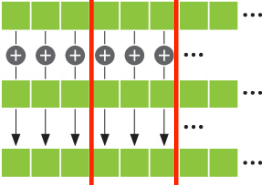
\includegraphics[width=0.3\linewidth]{figures/OpenMP/Distribute.png}
    \end{figure}
    \begin{verbatim}
        #pragma omp parallel shared (a, b)
        {
            int id, i, Nthrds, istart, iend;
            id = omp_get_thread_num();
            Nthrds = omp_get_num_threads();
            istart = id * N / Nthrds;
            iend = (id+1) * N / Nthrds;
            for(i=istart;i<iend;i++) { 
                a[i] = a[i] + b[i]; 
            }
        } 
    \end{verbatim}
\end{frame}

\begin{frame}[fragile]{Các mệnh đề schedule}
    Mệnh đề schdule được dùng để xác định cách chia vùng dữ liệu trong các vòng lặp giữa các luồng
    \begin{itemize}
        \item schedule (static | dynamic | guided [,chunk\_size])
        \item schedule (auto | runtime)
    \end{itemize}
    \begin{itemize}
        \item static chia các lặp lại của một vòng lặp thành các phần có kích thước bằng nhau và gán một phần cho mỗi luồng.
        Kích thước các phần được xác định tại thời điểm biên dịch và duy trì không đổi trong suốt quá trình thực thi của vòng lặp.
        \item dynamic gán các đoạn nhỏ của dữ liệu cho các luồng tại thời điểm chạy.
        Mỗi luồng thực hiện phần được gán và yêu cầu đoạn tiếp theo khi hoàn thành (các đoạn nhỏ kích thước bằng nhau).
        Kích thước các đoạn dữ liệu do từng luồng đảm nhận khác nhau.
        \item guided tương tự như dynamic nhưng các đoạn dữ liệu nhỏ do từng luồng đảm nhận giảm theo hàm mũ.
    \end{itemize}
\end{frame}

\begin{frame}[fragile]{Các mệnh đề schedule}

    \begin{itemize}
        \item auto cho phép OpenMP tự động chọn lịch trình phù hợp dựa trên điều kiện của runtime.
        Lịch trình được đưa ra bởi hệ thống.
        \item runtime cho phép lịch trình và chunk\_size xác định tại thời điểm chạy sử dụng biến môi trường.
    \end{itemize}
    \begin{verbatim}
#pragma omp parallel for schedule(static) private(id)
for(i = 0; i < N; i++) {
    A[i] = B[i] + C[i];
}
    \end{verbatim}
\end{frame}

\begin{frame}[fragile]{Chỉ thị sections}
    Mỗi section được gán cho một thread
    \begin{verbatim}
#pragma omp parallel
#pragma omp sections
{
    #pragma omp section
    printf("1 + 1, id: %d\n", omp_get_thread_num());
    #pragma omp section
    printf("1 + 2, id: %d\n", omp_get_thread_num());
    #pragma omp section
    printf("1 + 3, id: %d\n", omp_get_thread_num());
}
    \end{verbatim}

    Một barrier ngầm định ở cuối khối omp sections.
    Có thể tắt barrier sử dụng từ khóa nowait.
\end{frame}

\begin{frame}[fragile]{Chỉ thị sections}
    \begin{verbatim}
#pragma omp parallel private(id)
{
    int id = omp_get_thread_num();
    #pragma omp sections nowait
    {
        #pragma omp section
        printf("1 + 1, id: %d\n", id);
        #pragma omp section
        printf("1 + 2, id: %d\n", id);
        #pragma omp section
        printf("1 + 3, id: %d\n", id);
    }
    printf("%d\n", id);
}
    \end{verbatim}
\end{frame}

\begin{frame}[fragile]{Loop Collapse}
    \begin{itemize}
        \item Cho phép song song hóa giữa các vòng lặp lồng nhau mà không cần dùng song song hóa lồng nhau.
        \item Mệnh đề collapse chỉ thị bao nhiêu vòng lặp bị collapse
    \end{itemize}
    \begin{verbatim}
#pragma omp parallel for collapse(2)
for (i = 0; i < M; i++) {
    for (j = 0; j < P; j++) {
        int temp = 0;
        for (k = 0; k < N; k++) {
            temp += *(B + i * N + k) * *(C + k * P + j);
        }
        *(A + i * P + j) = temp;
    }
}
    \end{verbatim}
\end{frame}
\end{document}